\section{Evaluation}
\label{sec:eval}

We conducted experiments on Planet-Lab platform to evaluate
SMON. Planet-Lab is a global research network consisting of
900+ nodes at 400+ sites around the world.

We evaluate SMON by first study its performance, and we
focus on the performance of self-deployment and disabling a
deployed SMON system. In the evaluation, We confirm that the
overhead introduced in self-deployment is low. By comparing
the performance of SMON at different scales, we show that
SMON design achieves good scalability. At last, we show that
the load on authentication agent to solve the authentication
challenge is low and a single agent can support nearly 1000
SMON peers on a moderate PC machine.

%let SMON start self-deployment. We study the performance of
%the self-deployment process, and measure the overhead
%introduced in solving race conditions. To show SMON has
%good scalability, we deploy SMON on another set of 24
%nodes, and compare the performance with the previous
%deployment. We then close SMON by ... and study the
%performance ...
%
%Our experimental results show that SMON is efficient at
%deploying itself and achieves good scalability, the
%overhead caused by race condition is small and the active
%state transition is fast.

\subsection{Performance}

First we evaluate the performance of SMON. We concentrate on
two representative activities: deploying a new SMON system
and disabling it. We select 117 nodes on Planet-Lab, all of
which are university nodes in North America. To deploy a
SMON system, we use the client utility of SMON to deploy a
peer on \texttt{planet\-lab2.ucsd.edu} (shortened as
\texttt{ucsd2} node) and start it. Then SMON will deploy
itself to other 116 nodes automatically. After the
deployment is accomplished, we just disable it by issuing a
RPC call to \texttt{ucsd2} to set the \texttt{livetag} to
false.  The ping interval of the SMON peer is configured as
5 seconds.

\begin{figure}%[t]
\centering
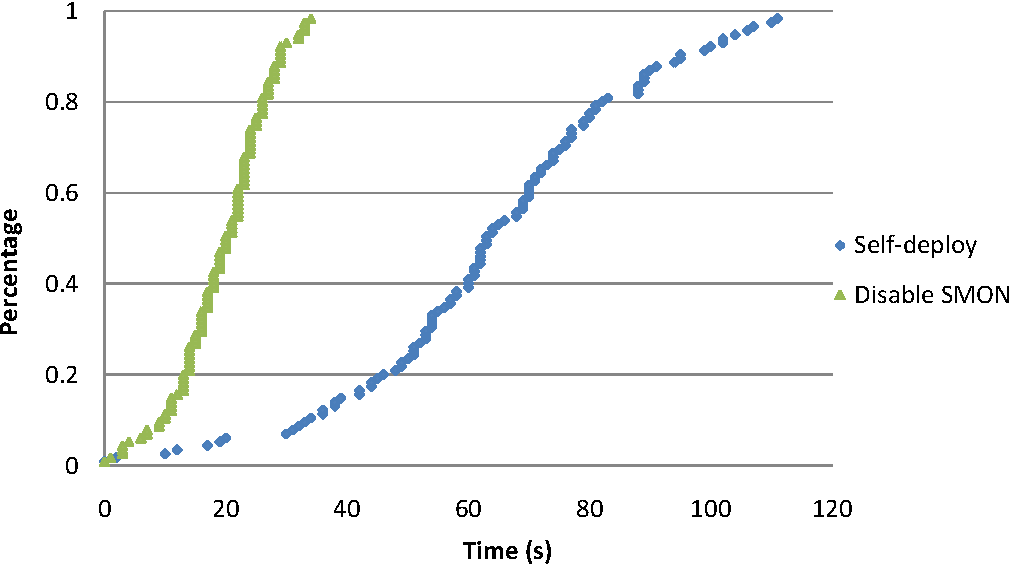
\includegraphics[width=\linewidth]{deploy_disable}
\caption{Deploy SMON on 117 nodes and then disable it.}
\label{fig:smonperf}
\end{figure}

Figure~\ref{fig:smonperf} summarizes the progress of
deploying and disabling SMON on 117 nodes, and they take
111 seconds and 34 seconds in total, respectively. The
progress curves show similar trends with analysis result
(Figure~\ref{fig:yr}). The difference in two curves are
mainly caused by the time cost to ``infect'' a new peer. It
takes longer time to deploy a new peer than to set
\texttt{livetag} of another peer to false. Our experience
of using SMON also shows that progress curve may exhibit
long tail when some nodes are less responsive because the
network connection to the nodes are slow or the nodes are
overloaded.

When SMON deploy itself, multiple peers may try to deploy
and start a new peer on the same nodes simultaneously. This
introduces some overhead, although only one peer is started
at last. In the analysis, we show that the average overhead
is a constant value of 1.582, and we validate the analysis
here. Table~\ref{tbl:overhead} summarized the statistics for
the overhead number. On most of nodes (72 of 117 nodes, or
64.54\%), there's exactly one deployment. The largest
overhead number is 23. On average, the overhead number is
1.88, with an error of 18.84\% comparing to analysis result.

\begin{table}[hb]
\centering
\begin{tabular}{|l|c|c|}
\hline
overhead & nodes & \% \\
\hline
1 & 72 & 61.54 \\
2 & 26 & 22.22 \\
3 & 12 & 10.26 \\
4 & 3 & 2.56 \\
5 & 2 & 1.71 \\
15 & 1 & 0.85 \\
23 & 1 & 0.85 \\
\hline
\end{tabular}
\caption{Overhead number distribution.}
\label{tbl:overhead}
\end{table}

\subsection{Scalability}

To evaluate the scalability of self-deployment process, we
deploy a new instance of SMON system at a different scale
(24 random nodes out of 117 nodes) and compare the
performance of self-deployment process.
Table~\ref{tbl:scalability} summarizes the statistics
results.  We can see from the table that the scalability is
good.  While scale difference between two systems is about
4.88 (117/24) times, the 90-percentile deployment time is
only 1.57 (91/58) times of difference, while the median
value is 1.31 (63/48) times of difference.  The above two
ratios is close to the ratio of logarithm of system scales
($\log 117 / \log 24 = 1.49$).

\begin{table}[h]
\centering
\begin{tabular}{|l|c|c|}
\hline
  & 24 nodes & 117 nodes\\
\hline
median & 48 sec & 63 sec \\
\hline
90\% percentile & 58 sec & 91 sec\\
\hline
Final & 61 sec & 111 sec\\
\hline
\end{tabular}
\caption{Comparison of self-deployment process at different
scales.}
\label{tbl:scalability}
\end{table}

\subsection{Load on authentication agent}

SMON employs an authentication agent to help peers
automatically log into another node to deploy a new peer or
recover a failed peer. It solves the authentication
challenge on behalf of the requested peer. Solving the
authentication challenge involves expensive computations and
it is a reasonable to ask whether the agent a possible
performance bottleneck.

\begin{figure}[h]
\centering
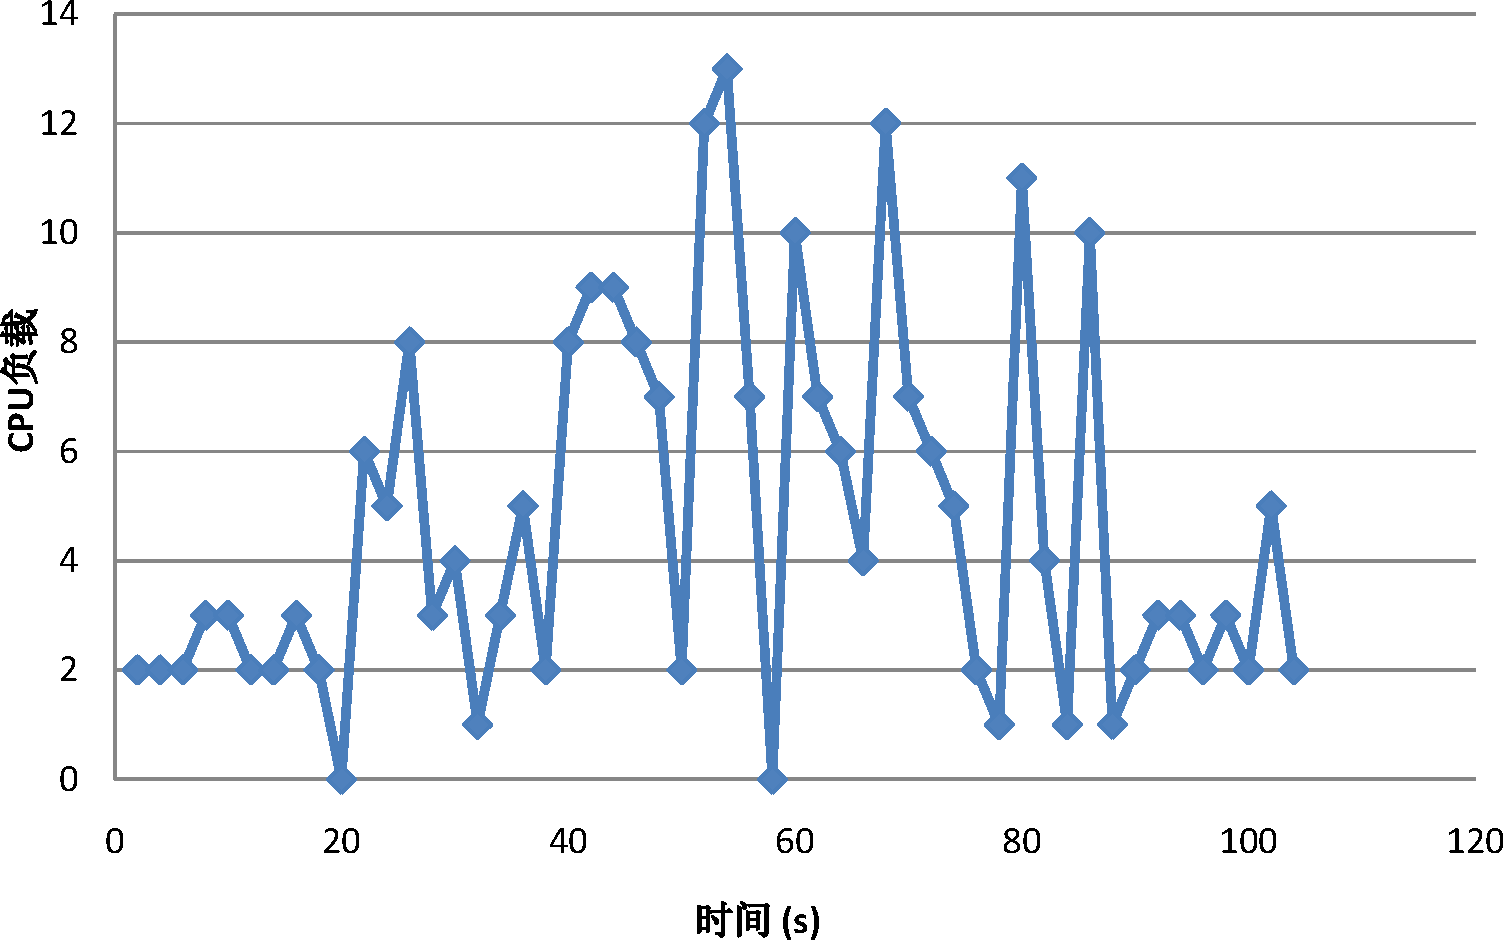
\includegraphics[width=\linewidth]{cpuload}
\caption{CPU load on authentication agent.}
\label{fig:agentload}
\end{figure}

We monitor the CPU usage on the authentication agent while
SMON is deploying itself to 117 nodes, and summarize the
result as figure~\ref{fig:agentload}. The authentication
agent runs on a PC machine of our lab. The PC is configured
with AMD Dual Core CPU 2.1GHz, 2GB memory and run Windows
XP.

It can be seen that the CPU load is about 13\% at maximum,
and usually below 10\%.  The load on the agent is
proportional to the frequency of authentication requests,
and the frequency reaches its maximum value when half of the
nodes are deployed with SMON peer. The maximum frequency is
also proportional to the scale of the nodes in theory. Thus
we can conclude that a single authentication agent is able
to support nearly a thousand of nodes to accomplish
self-deployment. After SMON is deployed, the frequency of
authentication requests depends on frequency of nodes
failures and is usually low.  And the agent could support
SMON at large scale without becoming a bottleneck.

% vim:foldmethod=marker:textwidth=60
